\section{}
Find the normal strain in the members $\overline{AB}$ and $\overline{BC}$ of the pin-connected plane structure shown in
Fig.(\ref{fig:q6problem}) if point B is moved leftward 2.5 mm. Assume that axial deformation is uniform throughout
the length of each member.


\begin{figure}[h]
    \centering
    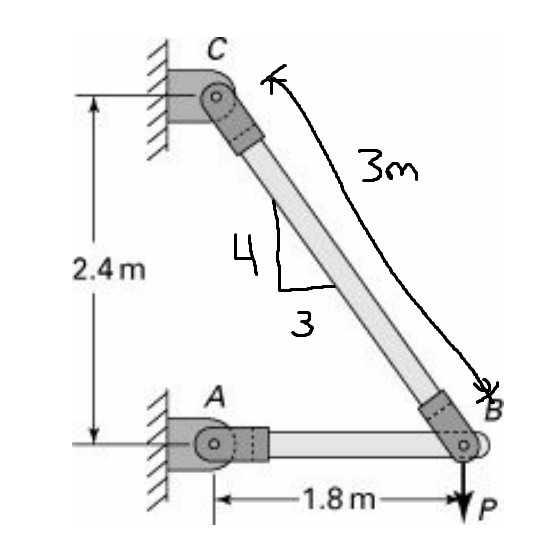
\includegraphics[width=0.3\linewidth]{Questions/Figures/Q6ProblemDiagram.png}
    \caption{Pin connected plane structure}
    \label{fig:q6problem}
\end{figure}

Convert the displacement of point B with respect to point A to a strain:
\begin{align*}
    \epsilon_{AB} &= \frac{\Delta L}{L} = \frac{-2.5 e-3}{1.8} = \boxed{\qty{-1.39e-3}{}}
\end{align*}

Find the displacement of point B with respect to point C:
\begin{align*}
    l_{BC, f} &= \sqrt{2.4^2 + (1.8 - 2.5\times 10^{-3})^2} = \qty{2.9985}{\meter} \\
    \Delta l_{BC} &= l_{BC, f} - l_{BC, i} = 2.9985 - 3.0 = \qty{-1.50 e-3}{\meter}
\end{align*}

Convert the displacement of point B with respect to point C to a strain:
\begin{align*}
    %\epsilon_{BC} &= \frac{\Delta L}{L} = \frac{-1.5 \times 10^{-3}}{3.0} = \boxed{-5.00 \times 10^{-4}}
    \epsilon_{BC} &= \frac{\Delta L}{L} = \frac{-1.5 e-3}{3.0} = \boxed{\qty{-5.00e-4}{}}
\end{align*}

